\documentclass{templateNote}
\usepackage{tcolorbox}
\usepackage{tabularx}
\usepackage{hyperref}
\usepackage{amsmath}
\usepackage{amssymb}
\usepackage{pdflscape}
\usepackage{tikz}
\usepackage{pdfpages}
\usepackage{soul}
\usepackage{media9}
\usepackage{adjustbox}
\usepackage{enumitem}
\usepackage{pdfpages}
\usepackage{mdframed} 
\usepackage{xcolor} 
% \usepackage[spanish,es-noquoting]{babel}

\begin{document}
% \linklogoU{https://www.ubiobio.cl/w/}
\linklogoD{https://github.com/NicoGomezM}
% \imagenlogoU{img/logo-ubb-txt-face.png}
\imagenlogoD{img/logoNGMFormal_sinF.png}
\titulo{Certamen 2}
\asignatura{Investigación de Operaciones}
\autor{
    Nicolás \textsc{Gómez Morgado}
}

\portada
\margenes
\tableofcontents
\newpage




\section{Materia}

\subsection{Cadenas de Markov}
\subsubsection{Proceso estocástico}
\noindent Es una sucesión $X_n$ de variables aleatorias, donde $n$ es un número entero no negativo. Se dice que $X_n$ es un proceso estocástico si para cada $n$, $X_n$ es una variable aleatoria.\\

\noindent\underline{\textbf{Ejemplo:}}

\noindent Supongamos que $X_n$ = Estado del clima en el dia $n$ = 1, 2, 3, ...\\ Supongamos que los estudios posibles son {n:nublado, s:soleado, r:lluvia}\\
\begin{center}
    $\Omega: {n,s,r}$ = Espacio muestral\\    
\end{center}

\noindent Realización de $X_n$:
\begin{center}
    $n,n,s,s,s,r,r,n,n,n;$
\end{center}

\noindent Supuestos para la cadena de Markov:
\begin{enumerate}
    \item El estado de la cadena en el instante $n+1$ depende solo del estado en el instante actual $n$ (no de anteriores[n-1,n-2,n-3...]).
    \item Con este supuesto se establecen las probabilidades condicionales homogéneas.\\
    $P_{ij}: $Probabilidad de pasar del estado i al estado j en una etapa. \\
    Notar que $P_{ij}$ no depende de $n$. \\
    Con esto se forma una matriz conformada por P = ($P_{ij})_{ij=1,2,3,...,*}$ \\
    P: Matriz de transición de probabilidades en una etapa.
    \item Supongamos que nuestros ejemplos:
    
    \begin{center}
        \[
        P =
        \begin{array}{l}
        \text{n} \\
        \text{s} \\
        \text{r} \\
        \end{array}
        \left(
        \begin{array}{ccc}
        P_{nn} & P_{ns} & P_{nr} \\
        P_{sn} & P_{ss} & P_{sr} \\
        P_{rn} & P_{rs} & P_{rr} \\
        \end{array}
        \right)
        \]
    \end{center}
    
    \begin{center}
        \[
        P = 
        \begin{array}{l}
        \text{n} \\
        \text{s} \\
        \text{r} \\
        \end{array}
        \left(
        \begin{array}{ccc}
        0.7 & 0.2 & 0.1 \\
        0.1 & 0.6 & 0.3 \\
        0.2 & 0.3 & 0.5 \\
        \end{array}
        \right)
        \]
    \end{center}

    Obs.: Cada pila es una distribución de probabilidad condicional.\\

    \text{\textbf{Probabilidad de pasar del estado i al estado j en una etapa:}}
    \begin{align*}
        \sum_{j}^{} P_{ij} = 1 - P_i
    \end{align*}

    \newpage
    \item Para cada cadena de Markov P tiene asociados un diagrama de transición entre estados.
    \begin{figure}[H]
        \centering
        \includegraphics[width=0.8\textwidth]{img/estados.png}
    \end{figure}
\end{enumerate}

\subsubsection{Clasificación de estados}
\begin{enumerate}
    \item \textbf{Estados comunicantes:} Dos estados i y j se dicen comunicantes si: $i \rightarrow j \land j \rightarrow i$\\
    \textbf{Obs.1:} La relación de comunicación es una relación de equivalencia.\\
    \textbf{Obs.2:} La relación i $\leftrightarrow$ j $\land$ j $\leftrightarrow$ k $\Rightarrow$ i $\leftrightarrow$ k
    \item \textbf{Clase de estados:} Una clase de estados es un subconjunto de estados que se comunican entre sí y no comunican con ningún estado fuera de la clase.
    \begin{itemize}
        \item \textbf{Estados recurrentes:} Un estado i se dice recurrente si la probabilidad de regresar a i en un número finito de pasos es 1.\\
        \textbf{Obs.:} Si un estado i es recurrente y se comunica con un estado j, entonces j es recurrente.
        \begin{itemize}[label=$\circ$]
            \item Aperiódico
            \item Periódico
        \end{itemize}
        \item \textbf{Estados transientes:} Un estado i se dice transitorio si la probabilidad de regresar a i en un número finito de pasos es menor que 1.\\
        \textbf{Obs.:} Si un estado i es transitorio y se comunica con un estado
        j, entonces j es transitorio.
        \item \textbf{Estados absorbentes:} Un estado i se dice absorbente si una vez que se llega a i, no se puede salir de él.
    \end{itemize}
\end{enumerate}

\subsubsection{Clases de cadenas}
\begin{enumerate}
    \item \textbf{Irreductible:} Se dice a una cadena irreductible si sus estados forman una sola clase. Pueden ser:
    \begin{itemize}
        \item Transiente
        \item Recurrente aperiódica
        \item Recurrente periódica
    \end{itemize}
    \item \textbf{Reductible:} Se dice a una cadena reductible si sus estados forman más de una clase.
\end{enumerate}

\subsubsection{Ergódica}
\noindent Una cadena de Markov se dice ergódica si es irreducible y recurrente aperiódica.\\
\textbf{Obs.:} Si una cadena de Markov es ergódica, entonces tiene una distribución límite.
\begin{itemize}
    \item Para determinar este tipo de cadenas podemos determinar el vector pi.
    \begin{align*}
        \vec{\pi} = (\pi_1, \pi_2, \pi_3, ..., \pi_k)  \quad &  \sum_{}^{}\pi_i = 1
    \end{align*}
\end{itemize}

\newpage
\section{Ejercicios Parte 1}

\begin{enumerate}
    \item Suponiendo que cada año el 50\% de los alumnos de primero pasa a segundo, el 30\% permanece primero y el 20\% abandona; de los alumnos de segundo el 50\% pasa a tercero, el 40\% permanece en segundo y el 10\% abandona, y de los alumnos de tercer curso el 60\% terminan o abandonan y el 40\% repiten tercero.Se pide:
    \begin{enumerate}[label=\alph*)]
        \item Escribir matriz de transición describiendo previamente los estados del proceso.
        
        Para este caso describiremos como el espacio muestral:
        \begin{center}
            $\Omega: {1,2,3}$ = Espacio muestral\\
        \end{center}
        \textit{Donde:}
        1: Primer Año; 2: Segundo Año; 3: Tercer Año

        \begin{table}[h]
            \centering
            \begin{tabular}{|r|c|c|c|}
            \hline
                                 & \textbf{Pasa}   & \textbf{Abandona}  & \textbf{Repite} \\ \hline
            \textbf{Primer Año } & 0.5             & 0.2                & 0.3 \\ 
            \textbf{Segundo año} & 0.5             & 0.1                & 0.4 \\ 
            \textbf{Tercer año } & 0               & 0.6                & 0.4 \\ \hline
            \end{tabular}
        \end{table}

        \begin{center}
            \[
            P = 
            \begin{array}{l}
            \text{1} \\
            \text{2} \\
            \text{3} \\
            \end{array}
            \left(
            \begin{array}{ccc}
                P_{1p} & P_{1a} & P_{1r} \\
                P_{2p} & P_{2a} & P_{2r} \\
                P_{3p} & P_{3a} & P_{3r} \\
            \end{array}
            \right)
            \]
        \end{center}
        \begin{center}
            \[
            P = 
            \begin{array}{l}
            \text{1} \\
            \text{2} \\
            \text{3} \\
            \end{array}
            \left(
            \begin{array}{ccc}
                0.5 & 0.2 & 0.3 \\
                0.5 & 0.1 & 0.4 \\
                0   & 0.6 & 0.4 \\
            \end{array}
            \right)
            \]
        \end{center}
        \item Si entran 600 alumnos un año en primer curso, calcular cuántos habrá en cada curso (de esos 600) al principio de tercer año.

        \begin{itemize}
            \item Primer año: 600 alumnos
            \begin{itemize}
                \item Primer curso: 
                \begin{itemize}
                    \item Pasa: 600 * 0.5 = 300
                    \item Abandona: 600 * 0.2 = 120
                    \item Repite: 600 * 0.3 = 180
                \end{itemize}
            \end{itemize}
            \item Segundo año
            \begin{itemize}
                \item Primer curso:
                \begin{itemize}
                    \item Pasa: 180 * 0.5 = 90
                    \item Abandona: 180 * 0.1 = 18
                    \item Repite: 180 * 0.4 = 72
                \end{itemize}
                \item Segundo curso:
                \begin{itemize}
                    \item Pasa: 300 * 0.5 = 150
                    \item Abandona: 300 * 0.1 = 30
                    \item Repite: 300 * 0.4 = 120
                \end{itemize}
            \end{itemize}
            \item Tercer año
            \begin{itemize}
                \item Primer curso:
                \begin{itemize}
                    \item Pasa: 72 * 0.5 = 36
                    \item Abandona: 72 * 0.1 = 7.2
                    \item Repite: 72 * 0.4 = 28.8
                \end{itemize}
                \item Segundo curso:
                \begin{itemize}
                    \item Pasa: 120 * 0.5 = 60
                    \item Abandona: 120 * 0.1 = 12
                    \item Repite: 120 * 0.4 = 48
                \end{itemize}
                \item Tercer curso:
                \begin{itemize}
                    \item Abandona: 150 * 0.6 = 90
                    \item Repite: 150 * 0.4 = 60
                \end{itemize}
            \end{itemize}
        \end{itemize}
        Por lo tanto al principio del tercer año tendremos 150 alumnos en tercer curso, 120 en segundo y 72 en primer curso.
        \item ¿Qué estados comunican entre sí?, ¿Es irreducible la cadena?, Indicar razonadamente qué estados son recurrentes y cuáles son transitorios.
        
        Según lo detallado en el siguiente grafo:

        \begin{figure}[H]
            \centering
            \includegraphics[width=0.5\textwidth]{img/ejer1.png}
        \end{figure}

        Los estados que se comunican entre si serian:
        \begin{itemize}
            \item Primer año $\rightarrow$ Segundo año
            \item Primer año $\rightarrow$ Primer año
            \item Segundo año $\rightarrow$ Tercer año
            \item Segundo año $\rightarrow$ Segundo año
            \item Tercer año $\rightarrow$ Tercer año
            \item Todos los años $\rightarrow$ Abandono
        \end{itemize}
        Por lo tanto la cadena no es irreductible, es reductible, ya que posee 3 estados transientes (1,2,3) y 1 estado absorbente (0).
        \item Calcular la distribución límite en el caso de que exista.
        
        Para este caso la cadena no es Ergódica, por lo que no posee distribución límite.
    \end{enumerate}

    \newpage
    \item Se considera la cadena de Markov con la siguiente matriz de probabilidades de transición:
    \begin{center}
        \[
        P = 
        \left(
        \begin{array}{cccc}
            0.4 & 0 & 0.6 & 0   \\
            0.5 & 0 & 0   & 0.5 \\
            0   & 0 & 0   & 1   \\
            0   & 0 & 0.5 & 0.5 \\
        \end{array}
        \right)
        \]
    \end{center}
    \begin{enumerate}[label=\alph*)]
        \item Representar esta cadena en un grafo cuyos vertices sean los cuatro estados y cuyos arcos representen las probabilidades de transición.

        \begin{figure}[H]
            \centering
            \includegraphics[width=0.5\textwidth]{img/ejer2.png}
        \end{figure}

        \item Estudiar si la cadena es irreducible y aperiódica, y si los estados son recurrentes o transitorios.

        \begin{itemize}
            \item $C_1$\{1\}: Recurrente periódico.
            \item $C_2$\{2\}: Transiente.
            \item $C_3$\{3,4\}: Recurrente aperiódico.
        \end{itemize}

        Para este caso la cadena no es irreducible ya que posee 3 tipos de estados diferentes.
        \item Calcular la distribución limite en caso de que exista.
        
        Para este caso no existe distribución límite. Ya que la cadena no es irreductible recurrente aperiódica.
    \end{enumerate}

    \newpage
    \item Una rata se mueve en el laberinto de la figura. Estando en cualquier comportamiento sale por cualquiera de sus puertas con la misma probabilidad. Escribir la matriz de probabilidades de transición.
    \begin{center}
        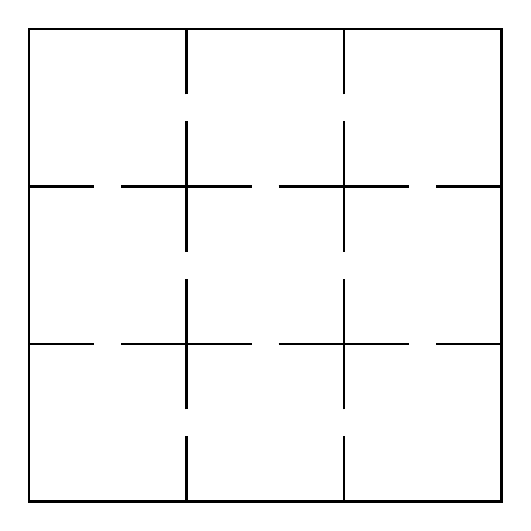
\begin{tikzpicture}
            % Dibuja el cuadrado exterior más pequeño
            \draw[line width=0.8pt] (0,0) rectangle (6,6);
            
            % Ajusta las divisiones verticales como puertas para el tamaño reducido
            % Puertas en la columna izquierda
            \draw[line width=1pt] (2,0) -- (2,0.83);
            \draw[line width=1pt] (2,1.17) -- (2,2.83);
            \draw[line width=1pt] (2,3.17) -- (2,4.83);
            \draw[line width=1pt] (2,5.17) -- (2,6);
            
            % Puertas en la columna derecha
            \draw[line width=1pt] (4,0) -- (4,0.83);
            \draw[line width=1pt] (4,1.17) -- (4,2.83);
            \draw[line width=1pt] (4,3.17) -- (4,4.83);
            \draw[line width=1pt] (4,5.17) -- (4,6);
            
            % Ajusta las divisiones horizontales como puertas para el tamaño reducido
            % Puertas en la fila inferior
            \draw[line width=1pt] (0,2) -- (0.83,2);
            \draw[line width=1pt] (1.17,2) -- (2.83,2);
            \draw[line width=1pt] (3.17,2) -- (4.83,2);
            \draw[line width=1pt] (5.17,2) -- (6,2);
            
            % Puertas en la fila media
            \draw[line width=1pt] (0,4) -- (0.83,4);
            \draw[line width=1pt] (1.17,4) -- (2.83,4);
            \draw[line width=1pt] (3.17,4) -- (4.83,4);
            \draw[line width=1pt] (5.17,4) -- (6,4);
        \end{tikzpicture}
    \end{center}

    La matriz correspondiente seria:

    \begin{center}
        \[
        P = 
        \begin{array}{l}
        \text{1} \\
        \text{2} \\
        \text{3} \\
        \text{4} \\
        \text{5} \\
        \text{6} \\
        \text{7} \\
        \text{8} \\
        \text{9} \\
        \end{array}
        \left(
        \begin{array}{ccccccccc}
            0 & 0.5 & 0 & 0.5 & 0 & 0 & 0 & 0 & 0\\
            0.33 & 0 & 0.33 & 0 & 0.33 & 0 & 0 & 0 & 0\\
            0 & 0.5 & 0 & 0 & 0 & 0.5 & 0 & 0 & 0\\
            0.33 & 0 & 0 & 0 & 0.33 & 0 & 0.33 & 0 & 0\\
            0 & 0.25 & 0 & 0.25 & 0 & 0.25 & 0 & 0.25 & 0\\
            0 & 0 & 0.33 & 0 & 0.33 & 0 & 0 & 0 & 0.33\\
            0 & 0 & 0 & 0.5 & 0 & 0 & 0 & 0.5 & 0\\
            0 & 0 & 0 & 0 & 0.33 & 0 & 0.33 & 0 & 0.33\\
            0 & 0 & 0 & 0 & 0 & 0.5 & 0 & 0.5 & 0\\
        \end{array}
        \right)
        \]
    \end{center}

    \newpage
    \item Determinar las clases y periodicidades de las cadenas con matrices de transición:
    \begin{enumerate}[label=\alph*)]
        \item
        \[
        P = \left(
        \begin{array}{cccc}
            0           & 0           & 1           & 0\\
            1           & 0           & 0           & 0\\
            \frac{1}{2} & \frac{1}{2} & 0           & 0\\
            \frac{1}{3} & \frac{1}{3} & \frac{1}{3} & 0\\
        \end{array}
        \right)
        \]
        \item
        \[
        P = \left(
        \begin{array}{cccc}
            0           & 1 & 0           & 0\\
            0           & 0 & 1           & 0\\
            0           & 1 & 0           & 0\\
            \frac{1}{3} & 0 & \frac{2}{3} & 0\\
        \end{array}
        \right)
        \]
    \end{enumerate}

    \newpage
    \item Calcula las participaciones en el mercado que a largo plazo alcanzarán las compañías R, S y T, si el comportamiento de los consumidores corresponde a una cadena de Markov con las probabilidades de cambio que se muestran en la tabla.
        \begin{center}
            \begin{tabular}{|c|c|c|c|}
                \hline
                von\textbackslash eu & \textbf{R} & \textbf{S} & \textbf{T} \\ \hline
                \textbf{R} & 0.6 & 0.1 & 0.3 \\
                \textbf{S} & 0.5 & 0.4 & 0.1 \\ 
                \textbf{T} & 0.2 & 0.1 & 0.7 \\ \hline
            \end{tabular}
        \end{center}
    
    \newpage
    \item Considerar el grafo adjunto. En cada iteración nos desplazamos con igual probabilidad a cada uno de los vertices adyacentes.
    \begin{center}
        \begin{tikzpicture}
            % Dibuja el cuadrado exterior
            \draw (0,0) rectangle (6,4);
            
            % Dibuja el triángulo invertido en el interior
            \draw (0,4) -- (3,2) -- (6,4);
            
            % Etiquetas en los vértices del cuadrado
            \node at (0,0) [below left] {D};
            \node at (6,0) [below right] {E};
            \node at (6,4) [above right] {B};
            \node at (0,4) [above left] {A};
            
            % Etiqueta en el vértice del triángulo
            \node at (3,2) [below] {C};
        \end{tikzpicture}
    \end{center}

    \begin{enumerate}[label=\alph*)]
        \item ¿Cuánto tiempo pasamos en A (a largo plazo)?
        \item Si comenzamos en A, ¿cuál es el número esperado de iteraciones hasta retornar a A?
        \item Si comenzamos en C, ¿cuál es el número esperado de pasos hasta llegar a A?
    \end{enumerate}

    \newpage
    \item Clasificar los estados de las cadenas de Markov con las siguientes matrices de transición:
    \begin{align*}
        P &= \left(
            \begin{array}{ccc}
                0 & 0.5 & 0.5 \\
                0.5 & 0   & 0.5 \\
                0.5 & 0.5 & 0   \\
            \end{array}
            \right)\\
    \end{align*}
    \begin{align*}
        P &= \left(
            \begin{array}{cccc}
                0   & 0   & 0.5 & 0.5\\
                1   & 0   & 0   & 0\\
                0   & 1   & 0   & 0\\
                0   & 1   & 0   & 0\\
            \end{array}
            \right)\\
    \end{align*}
    \begin{align*}
        P &= \left(
            \begin{array}{ccccc}    
                0.5 & 0.5 & 0   & 0   & 0\\
                0.5 & 0.5 & 0   & 0   & 0\\
                0   & 0   & 0.5 & 0.5 & 0\\
                0   & 0   & 0.5 & 0.5 & 0\\
                0.25& 0.25& 0   & 0   & 0.5\\
            \end{array}
            \right)\\
    \end{align*}

    \newpage
    \item En una población de 10,000 habitantes, 5000 no fuman, 2500 fuman uno o menos de un paquete diario y 2500 fuman más de un paquete diario. En un mes hay un 5\% de probabilidad de que un no fumador comience a fumar un paquete diario, o menos, y un 2\% de que un no fumador pase a fumar más de un paquete diario. Para los que fuman un paquete, o menos, hay un 10\% de probabilidad de que dejen el tabaco, y un 10\% de que pasen a fumar más de un paquete diario. Entre los que fuman más de un paquete, hay un 5\% de probabilidad de que dejen el tabaco y un 10\% de que pasen a fumar un paquete, o menos. ¿Cuántos individuos habrá de cada clase el próximo mes?
    
    \newpage
    \item Un agente comercial realiza su trabajo en tres ciudades A, B y C. Para evitar
    desplazamientos innecesarios está todo el día en la misma ciudad y allí
    pernocta, desplazándose a otra ciudad al día siguiente, si no tiene suficiente
    trabajo. Después de estar trabajando un día en C, la probabilidad de tener que
    seguir trabajando en ella al día siguiente es 0.4, la de tener que viajar a B es 0.4
    y la de tener que ir a A es 0.2. Si el viajante duerme un día en B, con
    probabilidad de un 20\% tendrá que seguir trabajando en la misma ciudad al día
    siguiente, en el 60\% de los casos viajará a C, mientras que irá a A con
    probabilidad 0.2. Por último si el agente comercial trabaja todo un día en A,
    permanecerá en esa misma ciudad, al día siguiente, con una probabilidad 0.1,
    irá a B con una probabilidad de 0.3 y a C con una probabilidad de 0.6.

    \begin{enumerate}[label=\alph*)]
        \item Si hoy el viajante está en C, ¿cuál es la probabilidad de que también tenga que trabajar en C al cabo de cuatro días?
        \item ¿Cuáles son los porcentajes de días en los que el agente comercial está en cada una de las tres ciudades?
    \end{enumerate}
    
    \newpage
    \item Suponga que toda la industria de refresco produce dos colas: Coca Cola y Pepsi Cola. Cuando una persona ha comprado Coca Cola hay una probabilidad de 90\% de que siga comprándola la vez siguiente. Si una persona compró Pepsi, hay 80\% de que repita la vez siguiente. Se pide:
    \begin{enumerate}[label=\alph*)]
        \item  Si una persona actualmente es comprador de Pepsi. ¿Cuál es la probabilidad de que compre Coca Cola pasadas dos compras a partir de hoy?
        \item Si en la actualidad una persona es comprador de Coca Cola. ¿Cuál es la probabilidad de que compre Coca Cola pasadas tres compras a partir de ahora?
        \item Supongamos que el 60\% de toda la gente toma hoy Coca Cola y el 40\% Pepsi. A tres compras a partir de ahora, ¿Qué fracción de los compradores estará tomando Coca Cola?.
    \end{enumerate}

\end{enumerate}

\newpage
\section{Ejercicios Parte 2}

\begin{enumerate}
    \item Estudiar las cadenas de Markov definidas por las matrices:
    
    \begin{align*}
        P_1 &= \left(
            \begin{array}{ccc}    
                0.4 & 0.6 & 0\\
                0.2 & 0.8 & 0\\
                0.3 & 0.2 & 0.5\\
            \end{array}
            \right)\\
    \end{align*}
    \textbf{Grafo de la matriz $P_1$:}
    \begin{figure}[H]
        \centering
        \includegraphics[width=0.5\textwidth]{img/ejer1_2.png}
    \end{figure}

    \begin{align*}
        P_2 &= \left(
            \begin{array}{ccc}    
                0   & 1   & 0  \\
                \frac{1}{4} & \frac{1}{4} & \frac{1}{2}  \\
                0 & \frac{1}{2} & \frac{1}{2}\\
            \end{array}
            \right)\\
    \end{align*}

    \begin{align*}
        P_3 &= \left(
            \begin{array}{cccc}    
                0.4&0.1&0.5&0\\
                0&0.5&0.2&0.3\\
                0.4&0.2&0&0.4\\
                0.5&0.1&0.3&0.1\\
            \end{array}
            \right)\\
    \end{align*}

    \begin{align*}
        P_4 &= \left(
            \begin{array}{cccc}    
                0.4&0.1&0.4&0.1\\
                0.1&0.2&0.2&0.5\\
                0.6&0&0.2&0.2\\
                0.2&0.4&0.1&0.3\\
            \end{array}
            \right)\\
    \end{align*}
    
    \begin{align*}
        P_5 &= \left(
            \begin{array}{ccc}    
                \frac{1}{4}   &  0  & \frac{3}{4}  \\
                \frac{1}{4} & \frac{1}{2} & \frac{1}{4}  \\
                \frac{1}{2} & 0 & \frac{1}{2}\\
            \end{array}
            \right)\\
    \end{align*}


    \newpage
    \item Considerar un proceso de Markov con la siguiente matriz de probabilidades de transición:
    \begin{align*}
    P_5 &= \left(
        \begin{array}{ccc}    
            \frac{1}{8}   &  \frac{1}{8}    & \frac{3}{4}  \\
            \frac{1}{2}   &  \frac{1}{4}    & \frac{1}{4}  \\
            \frac{3}{4}   &       0         & \frac{1}{4}\\
        \end{array}
        \right)\\
    \end{align*}

    \begin{enumerate}[label=\alph*)]
        \item Calcular el tiempo medio de primer paso de 3 a 2 ($\mu_{32}$).
    \end{enumerate}

    
    \newpage
    \item Un taller de reparaciones puede efectuar el trabajo A o el trabajo B, pero no los dos
    simultáneamente; la tarea A requiere 2 días y la B 1 día. Los posibles estados del taller son
    pues:

    \begin{center}
        \textbf{1} = ninguna tarea, \textbf{2} = primer día de la tarea A, \\\textbf{3} = segundo día de la tarea A, \textbf{4} = tarea B.
    \end{center}

    La probabilidad de una nueva demanda de tarea A al principio de cada día es “a”; la de la tarea B es “b”. 

    No hay colas, si el taller está a mitad de ejecución de una tarea A, la llegada de una nueva demanda se pierde. 

    La única ambigüedad se plantea cuando el taller termina un trabajo al final de un día y tiene la posibilidad de empezar al día siguiente con una tarea A o una B. Las dos políticas son posibles:

    \begin{enumerate}[label = \arabic*)]
        \item Empezar siempre con una tarea A con preferencia a una B.
        \item Empezar siempre con una tarea B con preferencia a una A.
    \end{enumerate}

    \begin{enumerate}[label = \alph*)]
        \item Demostrar que para la política 1 la matriz de probabilidades de transición es:
        \begin{align*}
            P &= \left(
                \begin{array}{cccc}    
                    (1-a)(1-b)  & a & 0 & b(1-a)\\
                    0           & 0 & 1 & 0     \\
                    (1-a)(1-b)  & a & 0 & b(1-a)\\
                    (1-a)(1-b)  & a & 0 & b(1-a)\\
                \end{array}
                \right)\\
        \end{align*}
        \item Encontrar la matriz de probabilidades de transición para la política 2.
    \end{enumerate}

    \newpage
    \item El siguiente proceso de Markov empieza en el estado 1
    \[
    P = \begin{pmatrix}
        0   & 0.5 & 0.5 \\
        0.4 & 0   & 0.6 \\
        0   & 0.2 & 0.8 \\
    \end{pmatrix}
    \]
    Encontrar las probabilidades de que:
    \begin{enumerate}[label=\alph*)]
        \item El proceso esté en el estado 3 después de tres transiciones.
        \item Después de la tercera transición desde el estado 3 hasta el 2 las dos transiciones siguientes
        sean ($2\rightarrow1\rightarrow3$) o ($2\rightarrow3\rightarrow3$).
        \item El proceso entre en el estado 2 exactamente una vez en las tres primeras transiciones.
        \item El proceso realice la transición $1\rightarrow2$ exactamente una vez en las tres primeras
        transiciones.
    \end{enumerate}


    \newpage
    \item Supongamos que la probabilidad de que mañana llueva si hoy está lloviendo es 0.6, y que
    la probabilidad de que mañana haga buen tiempo si hoy hace buen tiempo es 0.4
    \begin{enumerate}[label=\alph*)]
        \item Determinar la matriz de probabilidades de transición de la cadena de Markov
        correspondiente.
        \item Hallar la distribución de probabilidad del estado estacionario
    \end{enumerate}


    \newpage
    \item - Determinar las clases de las siguientes cadenas de Markov y decir si son o no recurrentes
    \begin{enumerate}[label=\alph*)]
        \item 
        \[
        P = \begin{pmatrix}
            0 & 0 & \frac{1}{3} & \frac{2}{3} \\
            1 & 0 & 0 & 0 \\
            0 & 1 & 0 & 0 \\
            0 & 1 & 0 & 0 \\
        \end{pmatrix}
        \]
        \item  
        \[
        P = \begin{pmatrix}
            1           & 0           & 0             & 0 \\
            1           & \frac{1}{2} & \frac{1}{2}   & 0 \\
            0           & \frac{1}{2} & \frac{1}{2}   & 0 \\
            \frac{1}{2} & 1           & 0             & \frac{1}{2}\\
        \end{pmatrix}
        \]
    \end{enumerate}


    \newpage
    \item Las familias de cierto país se clasifican según residan en áreas rurales, urbanas o
    suburbanas. Los estudios de movilidad demográfica estiman que, en promedio, en el curso de
    un año, el 15\% de las familias urbanas cambia de residencia y se traslada a un área suburbana,
    y el 5\% a un área rural; mientras que el 6\% de las familias residentes en áreas suburbanas se
    traslada a áreas urbanas, y el 4\% a áreas rurales, y finalmente el 4\% de las familias rurales
    migra a las áreas urbanas y el 6\% a las suburbanas.

    \begin{enumerate}[label=\alph*)]
        \item ¿Cuál es la probabilidad de que una familia que vive ahora en un área urbana siga viviendo
        en un área urbana dentro de dos años? ¿Y en una suburbana? ¿Y en una rural?
        \item Supongamos que en el presente el 40\% de las familias del país viven en áreas urbanas, el
        35\% en suburbanas y el 25\% en rurales. ¿Qué porcentaje de familias vivirá en áreas urbanas
        dentro de dos años?
        \item ¿Qué distribución de población es de prever en el futuro si las tendencias no cambian?
    \end{enumerate}
    

    \newpage
    \item - Un bosque consta de dos tipos de árboles: jóvenes (entre 0 y 3 mts de altura) y adultos (más
    de 3 mts). Cada año, el 30\% de los árboles jóvenes muere, el 10\% se vende por \$20 cada uno,
    el 20\% se mantiene entre 0 y 3 mts y el 40\% crece superando los 3 mts. Cada año, el 40\% de
    los árboles adultos se vende por \$50, el 20\% se vende por \$20, el 30\% permanece en el bosque
    y un 10\% muere.
    \begin{enumerate}[label=\alph*)]
        \item ¿Cuál es la probabilidad de que un árbol joven muera antes de ser vendido?
        \item Si plantar un árbol joven cuesta \$5, ¿cuál es el beneficio esperado para cada árbol joven plantado?
    \end{enumerate}


    \newpage
    \item Sea la siguiente matriz de probabilidades de transición: 
    \[
    P = \begin{pmatrix}
        0.5 & 0.3   & 0.2 \\
        0.2 & 0.15  & 0.65 \\
        0.1 & 0.1   & 0.8 \\
    \end{pmatrix}
    \]
    Con su vector de probabilidades iniciales $\vec{\pi}_{(0)} = (0.8,0.1,0.1)$
    Encontrar:
    \begin{enumerate}[label=\alph*)]
        \item El vector de probabilidades $\pi$ en el momento t = 2
        \item La probabilidad de que en los momentos t = 0, 1, 2, 3, la cadena asuma los estados 1, 3, 3, 2, respectivamente.
        \item El vector límite estacionario, si existe. 
        \item Dibujar el gráfico de estados.
    \end{enumerate}


    \newpage
    \item En cierta ciudad los habitantes pueden tener alguna de las profesiones A, B, C. En cada
    caso los hijos tienden a seguir la profesión del padre con probabilidades 3/5, 2/3 y 1/4
    respectivamente. Quienes no siguen la tradición del padre eligen equiprobable mente
    alguna de las otras dos.

    Hallar:

    \begin{enumerate}[label=\alph*)]
        \item La distribución porcentual de las profesiones en la próxima generación, si actualmente es de 20\% para A, 30\% para B y 50\% para C.
        \item La distribución límite de las generaciones cuando transcurren muchas generaciones. 
        \item Una cierta distribución porcentual de las profesiones que no cambie de una generación a otra.
    \end{enumerate}


    \newpage
    \item En la urna 1 tenemos 9 bolas blancas y 1 bola negra. En la urna 2 tenemos 9 bolas
    negras y una blanca. Extraemos una bola al azar de la urna 1. Si es negra, la regresamos a
    la urna. Si es blanca, la cambiamos por otra bola de la urna 2 que se extrae al azar. 

    Sea x(t), t = 0, 1, 2… el número de bolas en la urna 1 después de cada experimento. 

    \begin{enumerate}[label=\alph*)]
        \item Dibujar el gráfico de estados.
        \item Hallar distribución limite.
    \end{enumerate}

\end{enumerate}

\end{document}